\documentclass[11pt,letterpaper]{article}

% Please include your name below by replacing YOUR NAME HERE

%change to \templatetrue for template or \templatefalse for standalone problems
\newif \iftemplate \templatetrue

\usepackage{fullpage, color}
\usepackage{amsmath,amssymb,amsthm}
\usepackage{enumitem}
\newenvironment{solution}{\paragraph{Solution:}}{\hfill$\square$}
\usepackage{hyperref}
\usepackage{graphicx}

\newtheorem{lemma}{Lemma}
\newtheorem{theorem}[lemma]{Theorem}
\theoremstyle{definition}
\newtheorem{definition}{Definition}

% To define a lemma (or theorem or definition) use:
% \begin{lemma}
% Lemma statement
% \end{lemma}

% Include commands/ extra packages here, e.g.
\newcommand{\calA}{\mathcal{A}} % a popular adversary or algorithm
\newcommand{\N}{\mathbb{N}} % used for natural numbers




\bibliographystyle{plain}
\title{CS 5854 : Networks, Crowds, and Markets\\ Homework 2}
\author{Instructor: Rafael Pass\ \ \ \ \ \ TAs: Cody Freitag, Ben Chan
\medskip \\
Due: October 27, 2020, 11:59 pm Eastern Time
\bigskip \\ 
\iftemplate
YOUR NAME HERE
\fi
}
\date{}

\begin{document}
\maketitle

\iftemplate
\noindent 
\textbf{Collaborators:} I worked with \_ and \_. \\
\noindent
\textbf{Outside resources:} I used the following outside resources: \_. \\
\noindent
\textbf{Late days:} I have used \_ many late days on this assignment.
\bigskip
\fi

\iftemplate
\else
\noindent
\textbf{Homework Policies and Guidelines:}
\medskip

\begin{footnotesize}

\emph{\textbf{Submission:}} 
Your homework solutions must be \textbf{typed} and submitted
as a single .pdf file on Canvas. 
You must additionally submit a single .zip file containing all relevant files specified in 
the assignment for all coding problems.
Template .tex and .py files will be provided containing an outline for your submission.

\emph{\textbf{Late Days:}} 
Each student may use four ``late days" in total as desired throughout the semester, each of which grants a 24-hour extension to an assignment's 
due date. Late work beyond this limit will still be accepted and 
graded until grades have been released for that assignment, but (unless discussed in 
advance with the TA and/or instructor) will have a negative impact on final grades.

\emph{\textbf{Collaborations:}}
You may work in groups of up to \textbf{3} students. Every member of the group must list all other collaborators
at the top of their assignment. \emph{(Note: the maximum size of a connected component
of groups must be 3. If A,B, and C work together, it must not be the case that A and D work together.)}

Your submitted \textbf{answers, explanations, and discussion} for all written questions in the pdf \textbf{must be your own, individual, unique solutions}. You will receive \textbf{ZERO} points for written explanations which are copied verbatim or copied with minor changes (up to the discretion of the TAs)---either from another group member or from a \emph{cited} online source.
You \emph{may} share and even submit the same code, examples, figures, and graphs with your collaborators, but your explanations must be your own.
Additionally, you may make use of published material (papers, github, wikipedia, etc.), provided that you acknowledge and specifically cite all sources used.
Still, this does not give you permission to copy code/ explanations from an online source.
It is considered a violation of academic integrity to submit a problem solution that you are unable to explain orally to a member of the course staff.

\emph{\textbf{How to receive credit:}}
You must \textbf{justify all answers} to receive credit unless specified otherwise. We will do our best to make clear the level of justification we expect for each problem.
For coding questions, please turn in complete, executable code for each part of the question that asks 
for an implementation, and include a .txt file containing any required outputs if not already included in 
the main .pdf file. 
\emph{Using Python is required}. We will not grade code based on style, but we may mark down code if we are 
unable to understand what it is doing. You may use standard libraries to implement data structures 
such as graphs, but, unless otherwise specified, you may not use pre-existing implementations of any 
algorithms without express permission from the TAs. (If a problem asks you to implement X and you use a package that implements X for you, you will not get credit.)

\emph{\textbf{Grading:}} There will be four homeworks throughout the semester. Each homework (and each problem within each homework) will receive an associated weight specified by a number of points. Your raw score at the end of the semester will be the sum of points earned divided by the total number of available points. 
If your raw score is greater than 94\%, you are guaranteed to get at least an A, 90\% for A-, 87\% for B+, 84\% for B, and so on.
We reserve the right to lower the cutoffs (but we will not raise them).

There will additionally be optional bonus problems on some assignments. These will not be factored into your raw point totals, but will be factored in after computing your raw score to determine your final grade (for getting an A+, or possibly bumping up 1 or 2 letter grades).

\end{footnotesize}
\fi

\newpage

\noindent
{\Large\textbf{Part 1: Best-Response Dynamics}\par}

\begin{enumerate}

\item 
\begin{enumerate}
\item Let $G_1$ and $G_2$ be games with the same set of players and action sets for each player, and \emph{assume that BRD converges to a PNE} in both of these games. 
Consider a game $G = (G_1 + G_2)$ where each player plays a single action
for both $G_1$ and $G_2$ (i.e.\ plays the same action in both games at the same time) and receives utility equal to the \emph{sum} of the utilities they would earn from $G_1$ and $G_2$. \emph{Will BRD converge in this game?} If so, prove it; if not, find a counterexample and argue why it doesn't converge. 
\item Assume in a particular game $G = G_1 + G_2$ that BRD does converge. 
Will it necessarily converge to a state that is also a PNE in either $G_1$ or $G_2$? If so, prove it; if not, find a counterexample. 
\end{enumerate}

\iftemplate
\begin{solution}
\begin{enumerate}[label=(\alph*)]
\item 
\item 
\end{enumerate}
\end{solution}
\newpage
\fi

\item Consider the process of ``better-response dynamics" rather than BRD, where instead of choosing a player's best response (i.e. the response that maximizes their utility given others' actions), a player chooses any response that \emph{strictly} increases their utility given other players' actions.
\begin{enumerate}
\item Does the process of ``better-response dynamics" still converge in games for which there is an ordinal potential function $\Phi$? Prove it or show a counterexample. (\emph{Hint:} This is in the notes now. It suffices to reference the correct theorem.)
\item Can you think of a game for which BRD converges but ``better-response dynamics" might not? Show an example or justify that one doesn't exist. (\emph{Hint:} Remember that the better-response dynamics graph can have edges that the BRD graph might not. What if those edges formed a loop?)
\end{enumerate}

\item[*] \textbf{Bonus Question 1.} Recall the Traveler's Dilemma that we studied in chapter 1. We have already illustrated why BRD converges in this game; find a \textbf{weakly} ordinal potential function $\Phi$ over states of this game and use it to definitively prove the convergence of BRD. Make sure to justify that the potential function you find is weakly ordinal (you can do this via computer if you wish).

\item[*] \textbf{Bonus Question 1.5.} (\emph{This may be very difficult!}) Determine whether \emph{better-response dynamics} converge for the Traveler's Dilemma. No formal proof is necessary, and you need not come up with a potential function. You are free to either use simulations, show (experimentally) that the graph contains no cycle, or find an ordinal potential function and either prove it or experimentally verify.
\end{enumerate}

\iftemplate
\begin{solution}
\begin{enumerate}[label=(\alph*)]
\item 
\item 
\item[\textbf{Bonus 1}]
\item[\textbf{Bonus 1.5}]
\end{enumerate}
\end{solution}
\newpage
\fi


\noindent
{\Large\textbf{Part 2: Networked Coordination Games}\par}

\begin{enumerate}
\setcounter{enumi}{2}
\item Consider the following simple coordination game between two players:
\begin{center}
\begin{tabular}{|l|c|c|c|}
\hline
 & $(*, X)$ & $(*, Y)$\\
\hline
$(X, *)$ & $(x, x)$ & (0, 0)\\
\hline
$(Y, *)$ & (0, 0) & $(y, y)$\\
\hline
\end{tabular}
\end{center}
Show how we can pick $x$ and $y$ and then modify this payoff matrix by adding an intrinsic utility for a single player and a single choice (e.g. give player 1 some intrinsic utility for choice $Y$) such that the socially optimal state of the game is no longer an equilibrium.

\iftemplate
\begin{solution}
\end{solution}
\newpage
\fi

\item Consider a networked coordination game on a complete graph of five nodes. Assume for simplicity that all edges represent the same coordination game (that is, $Q_e (X, X) = Q_{e'} (X, X)$ for any pair of edges $e, e'$, and respectively for $Y$, but it is not necessarily the case that $Q_e (X, X) = Q_e (Y, Y)$), and that all nodes have the same intrinsic values for $X$ and $Y$ (that is, $R_i (X) = R_j (X)$ for any nodes $i, j$, and respectively for $Y$).
\begin{enumerate}
\item Can it be the case that every pure-strategy Nash equilibrium is socially optimal? If not, prove it. Otherwise, give a possible assignment of intrinsic and coordination utilities such that every pure-strategy Nash equilibrium of the resulting game is socially optimal (this requires finding all PNE and arguing that they give the maximum social welfare).

\item Is there a possible assignment of intrinsic and coordination utilities such that there exists a pure-strategy Nash equilibrium with social welfare less than half of the maximum attainable social welfare? If not, prove it. If so, show such an assignment and explain why your construction does not violate Theorem 4.5 from the notes (the price of stability). 
\end{enumerate}
\iftemplate
\begin{solution}
\begin{enumerate}[label=(\alph*)]
\item 
\item 
\end{enumerate}
\end{solution}
\newpage
\fi

\end{enumerate}

\noindent
{\Large\textbf{Part 3: Cascading Behavior in Networks}\par}

\begin{enumerate}
\setcounter{enumi}{4}
%EK, 19.8.3
\item Consider the network in Figure \ref{q7.fig}. Suppose that each node starts with the behavior $Y$, and has a $q = 2/5$ threshold for adopting behavior $X$. (That is, if at least 2/5 of a node's neighbors have adopted $X$, that node will as well.)
\begin{enumerate}
\item Let $e$ and $f$ form a set $S$ of initial adopters of $X$. Which nodes will eventually switch to $X$? (Assume that $S$ will not participate in BRD.)
\item Find a cluster of density $1 - q = 3/5$ in the part of the graph outside $S$ which blocks $X$ from spreading to all nodes starting from $S$.
\item Add one node to $S$ such that a complete cascade will occur at the threshold $q = 2/5$. Demonstrate how the complete cascade could occur (i.e. in what order nodes will switch).
\end{enumerate}
\begin{figure}
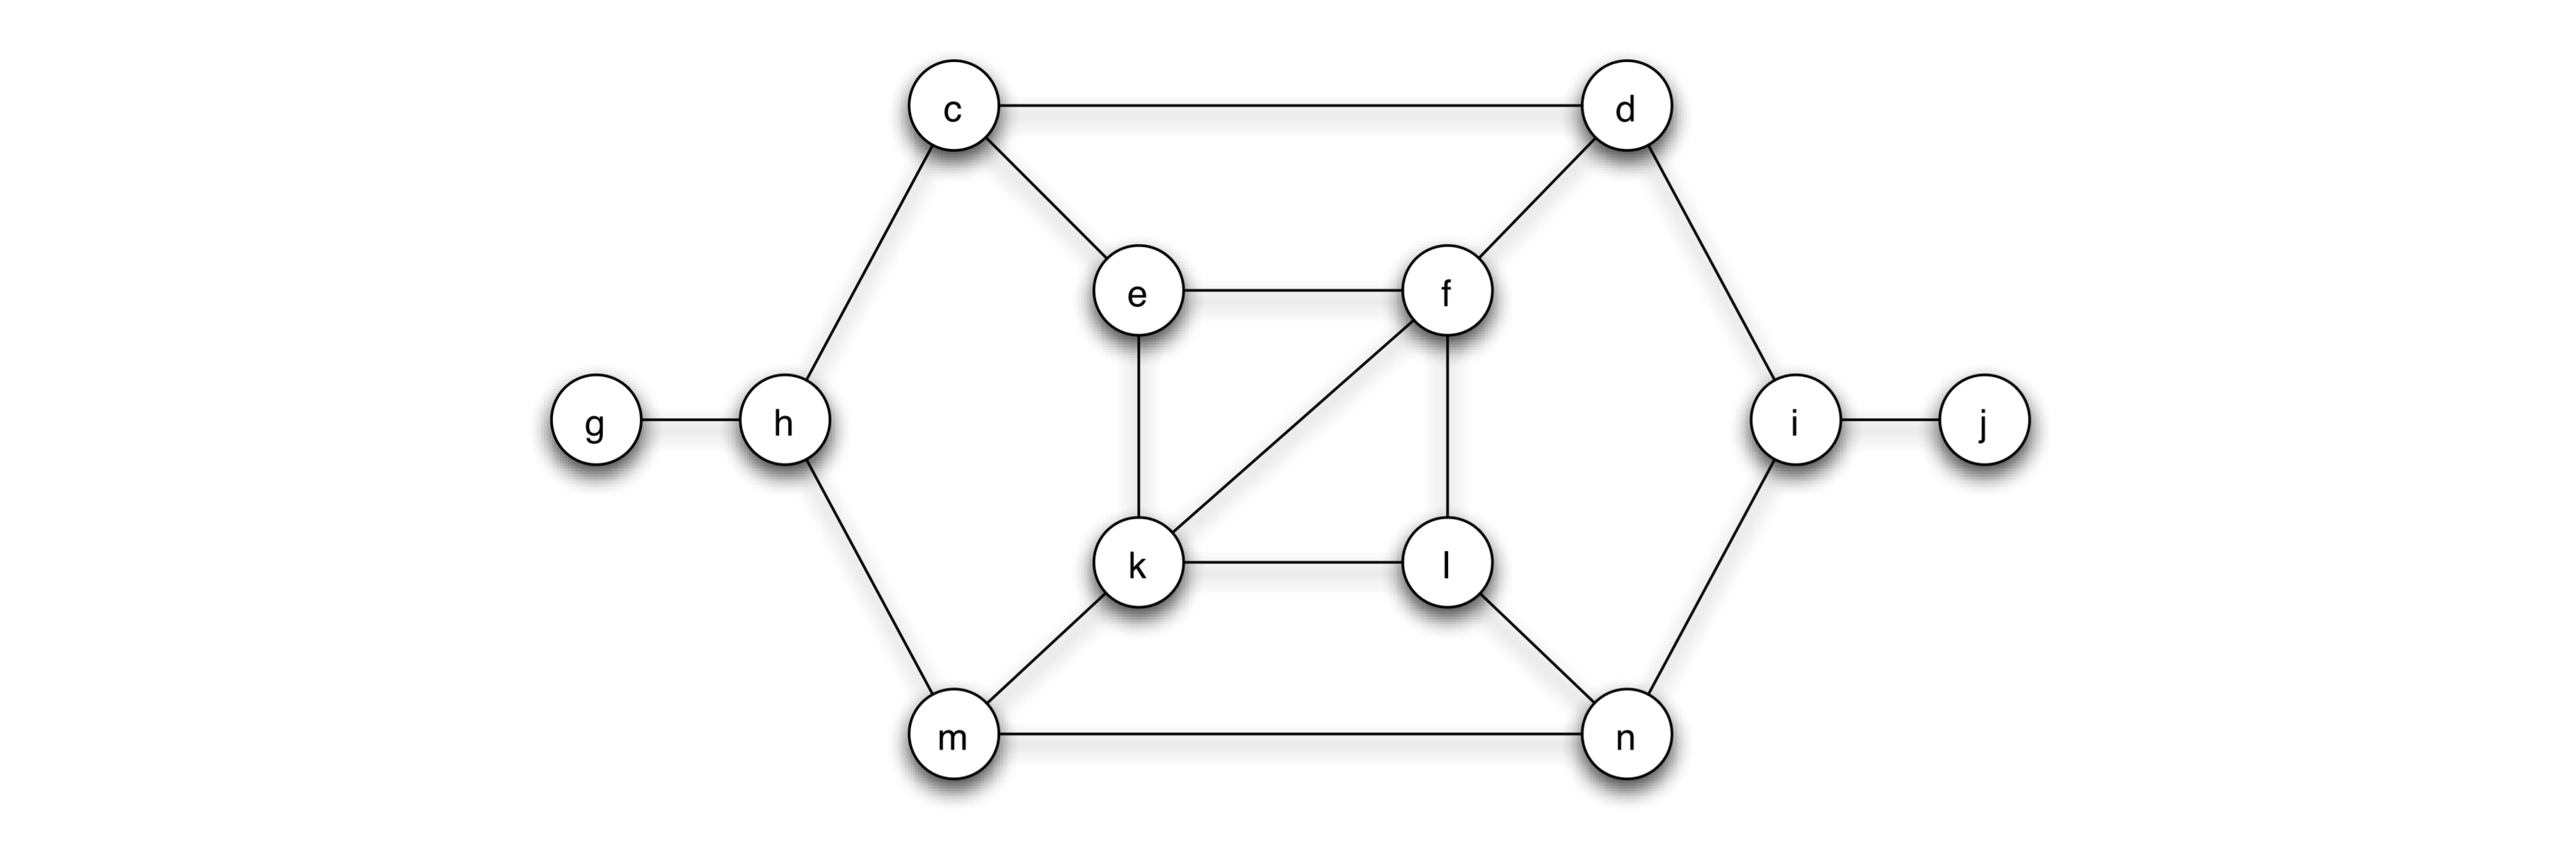
\includegraphics[width=\linewidth]{figure.jpg}
\caption{Question 5.}
\label{q7.fig}
\end{figure}

\iftemplate
\begin{solution}
\begin{enumerate}[label=(\alph*)]
\item 
\item 
\item
\end{enumerate}
\end{solution}
\newpage
\fi

\item 
\begin{enumerate}
\item Formulate a graph $G$, threshold $q$, and set $S$ of initial adopters such that, assuming we start with $S$ choosing $X$ (and, importantly, able to participate in BRD) and other nodes choosing $Y$, we can either end up with every node in $G$ playing $X$ or with every node in $G$ playing $Y$, depending on the order of switches in the BRD process.
\item What must be true of the set density of $S$ for the above property to hold?
\item What must be true of the set density in any subset of $V \setminus S$ for the above property to hold?
\end{enumerate}
\iftemplate
\begin{solution}
\begin{enumerate}[label=(\alph*)]
\item 
\item 
\item
\end{enumerate}
\end{solution}
\newpage
\fi
\end{enumerate}


\noindent
{\Large\textbf{Part 4: Traffic Networks}\par}

\begin{enumerate}
\setcounter{enumi}{6}
%EK, 8.4.2
\item There are two cities, A and B, joined by two routes which pass through towns C and D respectively. There are 120 travelers who begin in city A and must travel to city B, and may take the following roads:
\begin{itemize}
\item a local street from A to C with travel time $15 + x$, where $x$ is the number of travelers using it,
\item a highway from C to B with travel time 90,
\item a highway from A to D with travel time 90, and
\item a local street from D to B with travel time $15 + y$, where $y$ is the number of travelers using it.
\end{itemize}
\begin{enumerate}
\item Draw the network described above and label the edges with their respective travel times. The network should be a directed graph (assume that all roads are one-way). Note: you may just describe the graph if you are typing the assignment up. You may also include an image of the graph if that is easier for you.
\item Find the Nash equilibrium values of $x$ and $y$. (Show that this is the equilibrium.)
\item The government now adds a new \emph{two-way} road connecting the nodes where local streets and highways meet. This new road is extremely efficient and requires no travel time. Find the new Nash equilibrium.
\item What happens to the total travel time as a result of the availability of the new road? (You don't need to explain, a calculation is fine.)
\item Now suppose that the government, instead of closing the new road, decides to assign routes to travelers to shorten the total travel time. Find the assignment that minimizes the total travel time, and determine the total travel time using this assignment. (\emph{Hint:} It is possible to achieve a total travel time less than the original equilibrium. Remember that, with the new road, there are now four possible routes that each traveler can take.)
\end{enumerate}
\iftemplate
\begin{solution}
\begin{enumerate}[label=(\alph*)]
\item 
\item 
\item
\item
\item
\end{enumerate}
\end{solution}
\newpage
\fi
\end{enumerate}

\noindent
{\Large\textbf{Part 5: Experimental Evaluations}\par}

\medskip


\begin{enumerate}
\setcounter{enumi}{7}
\item 
This problem will make use of the data set available at:
 
[http://snap.stanford.edu/data/egonets-Facebook.html]. 

\medskip
In particular, please refer to the file ``facebook\_combined.txt.gz"; it contains a text file listing all 88,234 edges (\emph{undirected} edges representing Facebook friendship) in a sampled 4,039-node network (nodes are numbered 0 to 4038). It will be useful, for problem 8 to be able to input a graph presented in such a format into your code.

\begin{enumerate}
\item Consider the contagion examples that we observed in chapter 5 of the notes. Given an \emph{undirected} graph, a set of early adopters $S$, and a threshold $q$ (such that a certain choice $X$ will spread to a node if more than $q$ fraction of its neighbors are playing it), produce an algorithm that permanently infects the set $S$ of early adopters with $X$ and then runs BRD on the remaining nodes to determine whether, and to what extent, the choice will cascade through the network. (\emph{Note:} ``BRD" in this case is simply the process of iteratively deciding whether there is a node that will switch its choice and performing this switch.) 

Once again, turn in your code and verification that your algorithm works on a few simple test cases. In particular, include the output on the two examples from Figure 4.1 in the notes; let $S$ be the set of nodes choosing $X$ in the figure, and, for each of the two graphs, include one example with a complete cascade and one without one (and specify what value of $q$ you used for each).
\item Run your algorithm several (100) times on a fairly small random set of early adopters ($k = 10$) with a low threshold ($q = 0.1$) on the Facebook data set. What happens? Is there a complete cascade? If not, how many nodes end up being ``infected" on average?
\item Run your algorithm several (10) times with different values of $q$ (try increments of 0.05 from 0 to 0.5), and with different values of $k$ (try increments of 10 from 0 to 250). Observe and record the rates of ``infection" under various conditions. What conditions on $k$ and $q$ are likely to produce a complete cascade in this particular graph, given your observations?
\item[*] \textbf{Bonus Question 2.} (Optional, extra credit awarded depending on quality of solution.) Design an algorithm that, given a graph and a threshold $q$, finds (an approximation of) the smallest possible set of early adopters that will cause a complete cascade. Try running it on the Facebook data with different values of $q$ and seeing how large a set we need.
\end{enumerate}

\iftemplate
\begin{solution}
\begin{enumerate}[label=(\alph*)]
\item \textbf{Output for Figure 3.1a:} \\
\textbf{Output for Figure 3.1b:}
\item 
\item
\end{enumerate}
\end{solution}
\newpage
\fi

\item Consider the following problem: There are $n$ Uber drivers and $m$ potential riders. At a fixed point in time, each driver has a list of compatible riders that she can pick up. Our goal will be to match drivers to riders such that the most riders at this time are picked up. We will use the maximum-flow algorithm, described in Chapter 6 of the notes to do this.
\begin{enumerate}
\item First, implement an algorithm that, given a \emph{directed} graph, a source $s$, a sink $t$, and edge capacities over each edge in $E$, computes the maximum flow from $s$ to $t$ (you must implement this algorithm yourself). Turn in your code and verify that your algorithm works on a few simple test cases. In particular, test your algorithm on the graphs in Figures 6.1 and 6.3 from the lecture notes and submit the output. 
\item Given a set of $n$ drivers, $m$ riders, and sets of possible riders that each driver can pick up, 
\begin{enumerate}
\item explain how we can use this maximum-flow algorithm to determine the the maximum \emph{number} of matches, and
\item explain how we can additionally extend this to actually find the matchings.
\end{enumerate}
(\emph{Hint:} See the notes if you are confused about how to do this.)
\item Implement a maximal matching algorithm for Uber drivers and riders. Specifically, given $n$ drivers with constraints specified on $m$ riders, computed the assignments of drivers to riders. Test your algorithm on at least 2 examples (with at least $5$ riders and drivers each). Explain your examples and your results.
\item Now consider the case where there are $n$ drivers and $n$ riders, and the drivers each driver is connected to each rider with probability $p$. Fix $n = 1000$ (or maybe 100 if that's too much), and estimate the probability that all $n$ riders will get matched for varying values of $p$. Plot your results.
\item[*] \textbf{Bonus Question 3:} In the above example, let $p^*(n)$ be the smallest value of $p$ where all $n$ riders get matched with at least 99\% probability. Prove bounds on what $p^*(n)$ is as a function of $n$, e.g.\ is $p^*(n) \ge 1/n$ or $p^*(n) \le 1/2$. You will get partial credit for providing experimental evidence towards a proposed idea.
\end{enumerate}

\iftemplate
\begin{solution}
\begin{enumerate}[label=(\alph*)]
\item 
\textbf{Output for Figure 6.1:} \\
\textbf{Output for Figure 6.3:}
\item 
\item
\item 
\end{enumerate}
\end{solution}
\newpage
\fi


\end{enumerate}


\end{document}

